\begin{frame}{Messprinzip}
  \begin{columns}[c, onlytextwidth]
    \begin{column}{0.5\textwidth}
      \newcommand{\viewangle}{19.471220634490692}
\newcommand{\cloudangleA}{79.5}
\newcommand{\cloudangleB}{-40.7}
\begin{tikzpicture}[
    hydrogen/.style={fill, anchor=center, black!20,
    cloud, draw, cloud puffs=11, minimum size=0.5cm,
    cloud puff arc=120, aspect=3, inner sep=0em}
]
  \draw[thin] (0, 0) circle [radius = 1];
  \draw[thin] (0, 0) circle [radius = 2];
  \draw[thin] (0, 0) circle [radius = 3];
  \node[hydrogen]  at (\viewangle:1cm) {};
  \node[hydrogen]  at (\cloudangleA:2cm) {};
  \node[hydrogen]  at (\cloudangleB:2cm) {};
  \draw[darkred, ->, dashed, thick] (0, 3) -- +(-90+\viewangle:6.5cm);
  \filldraw (0, 0) circle [radius=2pt];
  \filldraw (0, 3) circle [radius=2pt] node[above] {Sonnensystem};
  \draw[->, thick, blue] (\cloudangleA:2cm) -- +(\cloudangleA-90:1cm) node[above, midway] {$v_1$};
  \draw[->, thick, blue] (\cloudangleA:2cm) -- +(\viewangle-90:0.55cm);
  \draw[->, thick, green] (\viewangle:1cm) -- +(-90+\viewangle:1.2cm) node[right, midway] {$v_2$};
  \draw[->, thick, red] (\cloudangleB:2cm) -- +(\cloudangleB-90:1cm) node[anchor=south east, midway] {$v_3$};
  \draw[->, thick, red] (\cloudangleB:2cm) -- +(\viewangle-90:0.49cm);
\end{tikzpicture}

    \end{column}
    \begin{column}{0.5\textwidth}
      \begin{tikzpicture}%
        \begin{axis}[%
            xmin=21.1,
            xmax=21.13,
            ymin=0,
            % ymax=120,
            width=\linewidth-12.05pt,
            xlabel={\SIQ{λ}{\centi\meter}},
            ylabel={$I$ / a.\,u.},
            extra x ticks={21.10611405413},
            extra x tick labels={$\mathrm{H}$},
          ]%
          \addplot[
            green,
            domain=21.1:21.13,
            samples=201,
          ]{0.6*exp(-0.5*(x-21.122)^2/(0.002^2))/(sqrt(2*pi*0.002^2))};
          \addplot[
            red,
            domain=21.09:21.12,
            samples=201,
          ]{0.6*exp(-0.5*(x-21.112)^2/(0.002^2))/(sqrt(2*pi*0.002^2))};
          \addplot[
            blue,
            domain=21.09:21.12,
            samples=201,
          ]{0.6*exp(-0.5*(x-21.110)^2/(0.002^2))/(sqrt(2*pi*0.002^2))};
        \end{axis}%
      \end{tikzpicture}%
    \end{column}
  \end{columns}
\end{frame}

\begin{frame}{Messprinzip}
  \begin{columns}[c, onlytextwidth]
    \begin{column}{0.5\textwidth}
      \newcommand{\viewangle}{19.471220634490692}
\begin{tikzpicture}
  \draw[thin] (0, 0) circle [radius = 1];
  \draw[thin] (0, 0) circle [radius = 2];
  \draw[thin] (0, 0) circle [radius = 3];
  \filldraw[darkred!30] (0, 3) -- (0, 2.3) arc [start angle=270, end angle=270+\viewangle, radius=0.7cm] -- cycle;
  \node[fill, anchor=center, black!20,
    cloud, draw, cloud puffs=11, minimum size=0.5cm,
    cloud puff arc=120, aspect=3, inner sep=0em]  at (\viewangle:1cm) {};
  \draw[darkred, ->, dashed, thick] (0, 3) -- +(-90+\viewangle:6.5cm);
  \draw (0, 0) -- + (0, 3) node[midway,left] {$R_0$};
  \draw (0, 0) -- (\viewangle:1cm) node[midway,below] {$R$};
  \filldraw (0, 0) circle [radius=2pt];
  \filldraw (0, 3) circle [radius=2pt] node[above] {Sonnensystem};
  \draw[->, thick] (0, 3) -- + (1, 0) node[below, right] {$v_0$};
  \draw[->, thick] (0, 3) -- + (\viewangle - 90:0.333);
  \draw[->, thick] (\viewangle:1cm) -- +(-90+\viewangle:1cm) node[right, midway] {$v$};
  \node[left] at (0, 2.65) {$γ$};
\end{tikzpicture}

    \end{column}
    \begin{column}{0.5\textwidth}
      \begin{enumerate}
        \item Messung der Doppler-Verschiebung der \SI{21}{\centi\meter}-Linie
          in eine Richtung
        \item Berechne für $v_{\max}$ = maximale Geschwindigkeit:
          \belowdisplayskip=0ex
          \begin{align*}
            R &= R_0 \cdot \sin{γ} \\
            v &= v_{\max} + v_0 \cdot \sin{γ} 
          \end{align*}
        \item Für Milchstraße:
          \begin{align*}
            v_0 = \SI{220}{\kilo\meter\per\second} \\
          R_0 = \SI{8.5}{\kilo pc}
          \end{align*}
      \end{enumerate}
    \end{column}
  \end{columns}
\end{frame}

\begin{frame}{LAB-Messung}
  Leiden/Dwingeloo – Argentinien – Bonn \cite{lab-kalberla}
  \begin{description}[Ortsauflösung]
    \item[2005] Veröffentlichung der Daten von zwei Teleskopen für den ganzen Himmel
    \item[1989--1993] \SI{30}{\meter}-Teleskop Argentinien
    \item[1994--2000] \SI{25}{\meter}-Teleskop Dwingeloo
    \item[Bonn] Zusammenfassung und Kalibrierung
    \item[Ortsauflösung] \SI{0.5}{\degree}
    \item[$\textcolor{darkred}{v}$-Auflösung] \SI{1.3}{\kilo\meter\per\second}
    \item[$\textcolor{darkred}{\TB}$-Auflösung] \SI{0.07}{\kelvin}
  \end{description}
  Frei zugänglicher Datensatz $\TB(l,b,v)$ mit $\approx \num{2e6}$ Datenpunkten
\end{frame}


\begin{frame}{Die \SI{21}{\centi\meter}-Linie – Vermessung der Milchstraße}%
  \begin{columns}[c, onlytextwidth]%
    \begin{column}{0.47\textwidth}%
      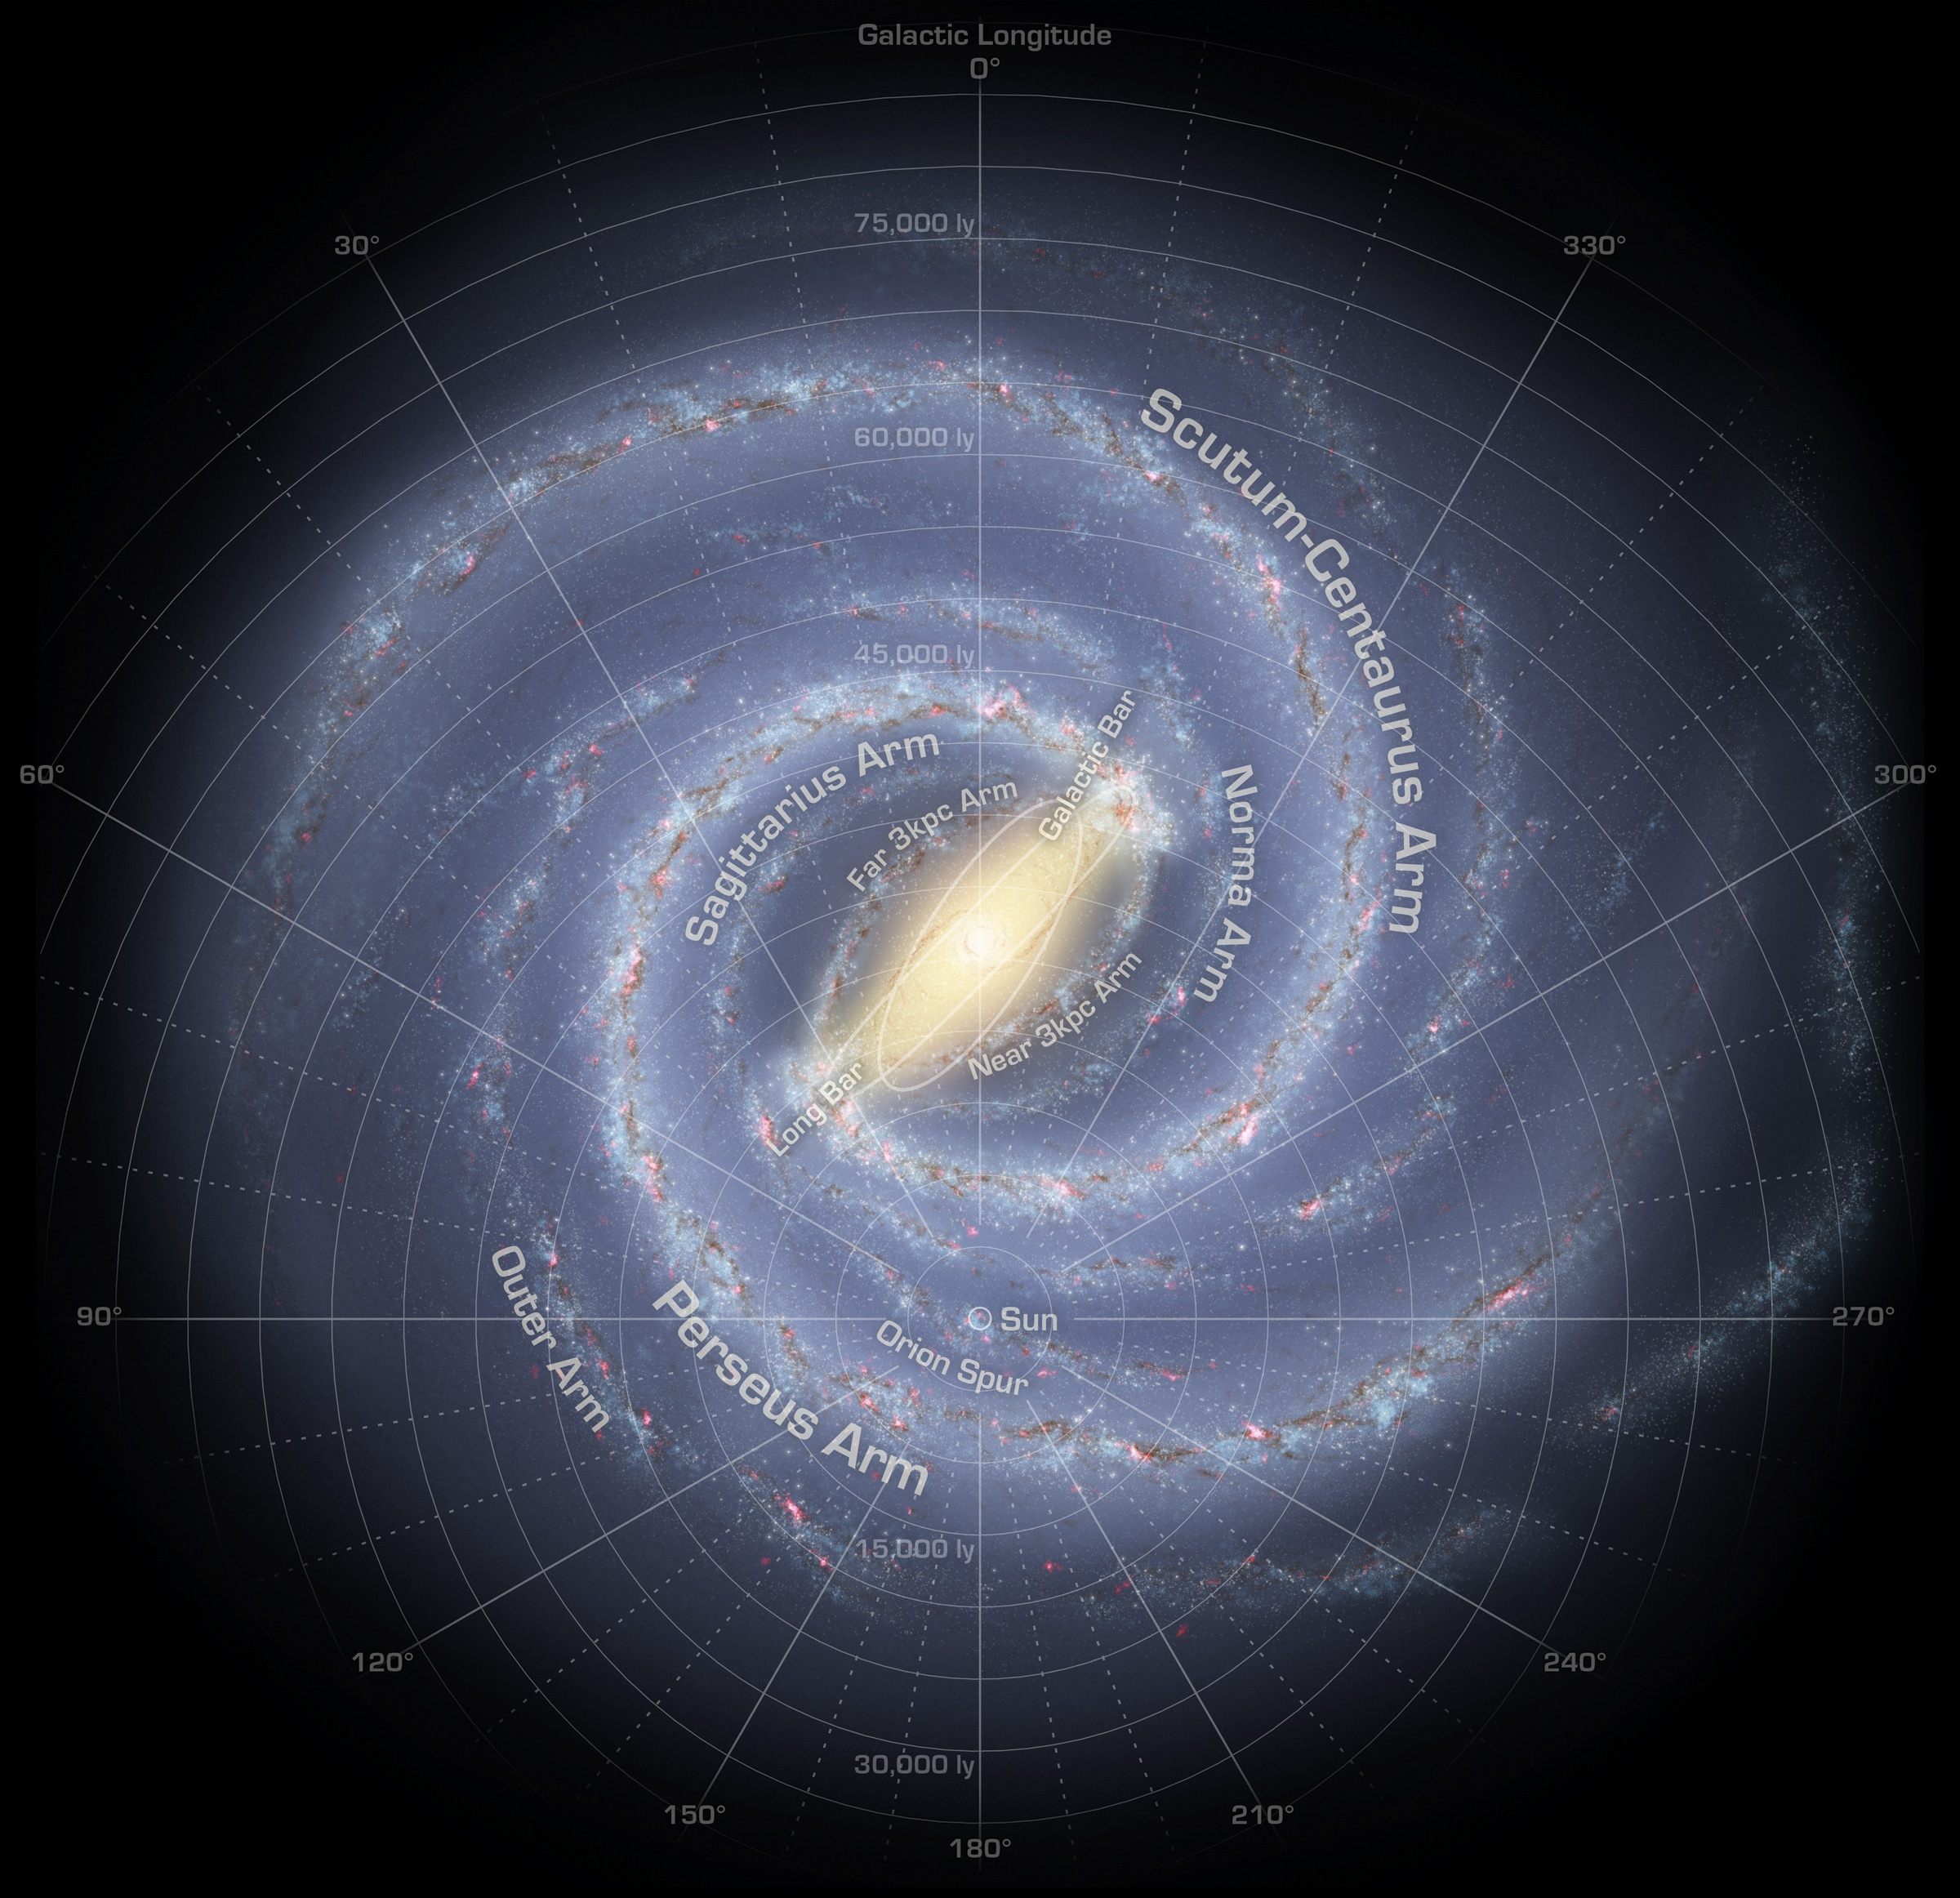
\includegraphics[width=\linewidth]{images/milkyway_structure_big_crop.jpeg}%
      \begin{tikzpicture}[overlay, remember picture, shift={(current page.center)}]%
        \only<1>{\draw[red!70!black, thick, o->] (-3.753, -1.41) -- +(65:4.5);}%
        \only<2>{\draw[red!70!black, thick, o->] (-3.819, -1.32) -- +(0:4.5);}%
      \end{tikzpicture}%
    \end{column}%
    \begin{column}{0.47\textwidth}%
      \begin{tikzpicture}%
        \begin{axis}[%
            title={$\TB$ für $l=\only<1>{\SI{335}{\degree}}\only<2>{\SI{270}{\degree}}$, \cite{lab-profile}},
            xmin=21.09,
            xmax=21.12,
            ymin=-10,
            ymax=120,
            width=0.93\linewidth,
            xlabel={\SIQ{λ}{\centi\meter}},
            ylabel={$\SIQ{\TB}{\kelvin}$},
            extra x ticks={21.10611405413},
            extra x tick labels={$\mathrm{H}$},
          ]%
          \only<1>{%
            \addplot[red!70!black] table[x index=3, y index=1]{./data/radial_velocity_l335.txt};%
          }
          \only<2>{%
          \addplot[red!70!black] table[x index=3, y index=1]{./data/radial_velocity_l270.txt};%
          }
        \end{axis}%
      \end{tikzpicture}%
    \end{column}%
  \end{columns}%
\end{frame}

\fullscreenimage[\cite{lab-survey}]{images/lab_survey.jpg}
